% ============================================================================
%  学生版讲义样式（整册小册子，可以写字的版本）
% ----------------------------------------------------------------------------
%  用法：主文件 03-讲义/讲义-学生版.tex 已经写好，一般不用动。
%        每课一个文件放在 03-讲义/学生版/ 下，开头写
%            \xhlesson{课次}{课题}{本课信息}
%        主文件里用 \input 引进来。
%  编译：XeLaTeX，编译两遍（目录需要第二遍才正确）
% ----------------------------------------------------------------------------
%  设计原则：留足空白，能写能画。
%    方框： mubiao 本课目标 / definition 定义 / dingli 定理 / example 例
%           sikao 想一想 / dongshou 动手做 / xiaojie 我学到了什么
%    留白： \liukong{行数} 画几道横线，给学生写字
% ============================================================================

% ---------------- 字体（跨平台自动选）----------------
\IfFontExistsTF{SimSun}{
  \setCJKmainfont{SimSun}[BoldFont=SimHei,ItalicFont=KaiTi,BoldItalicFont=SimHei]
  \setCJKsansfont{Microsoft YaHei}
  \setCJKmonofont{FangSong}
  \setCJKfamilyfont{zhsong}{SimSun}
  \setCJKfamilyfont{zhhei}{SimHei}
  \setCJKfamilyfont{zhkai}{KaiTi}
  \setCJKfamilyfont{zhfs}{FangSong}
}{
  \IfFontExistsTF{Songti SC}{
    \setCJKmainfont{Songti SC}[BoldFont=Heiti SC,ItalicFont=Kaiti SC,BoldItalicFont=Heiti SC]
    \setCJKsansfont{PingFang SC}
    \setCJKmonofont{STFangsong}
    \setCJKfamilyfont{zhsong}{Songti SC}
    \setCJKfamilyfont{zhhei}{Heiti SC}
    \setCJKfamilyfont{zhkai}{Kaiti SC}
    \setCJKfamilyfont{zhfs}{STFangsong}
  }{
    \setCJKmainfont{FandolSong-Regular.otf}[BoldFont=FandolHei-Regular.otf,ItalicFont=FandolKai-Regular.otf,BoldItalicFont=FandolHei-Regular.otf]
    \setCJKsansfont{FandolHei-Regular.otf}
    \setCJKmonofont{FandolFang-Regular.otf}
    \setCJKfamilyfont{zhsong}{FandolSong-Regular.otf}
    \setCJKfamilyfont{zhhei}{FandolHei-Regular.otf}
    \setCJKfamilyfont{zhkai}{FandolKai-Regular.otf}
    \setCJKfamilyfont{zhfs}{FandolFang-Regular.otf}
  }
}
\providecommand{\songti}{}\renewcommand{\songti}{\CJKfamily{zhsong}}
\providecommand{\heiti}{}\renewcommand{\heiti}{\CJKfamily{zhhei}}
\providecommand{\kaishu}{}\renewcommand{\kaishu}{\CJKfamily{zhkai}}
\providecommand{\fangsong}{}\renewcommand{\fangsong}{\CJKfamily{zhfs}}
\IfFontExistsTF{TeX Gyre Pagella}{%
  \setmainfont{TeX Gyre Pagella}%
}{\setmainfont{Latin Modern Roman}}

% ---------------- 宏包 ----------------
\usepackage[a4paper,left=2.1cm,right=2.1cm,top=2.3cm,bottom=2.1cm,headheight=15pt]{geometry}
\usepackage{amsmath,amssymb,mathtools,bm}
\usepackage{booktabs,array,multirow}
\PassOptionsToPackage{dvipsnames,svgnames}{xcolor}
\usepackage{graphicx,tikz}
\usetikzlibrary{calc}
\usepackage{enumitem}
\usepackage{fancyhdr}
\usepackage[many]{tcolorbox}
\tcbuselibrary{breakable,skins}
\usepackage[hidelinks]{hyperref}

% ---------------- 图片搜索路径 ----------------
\graphicspath{{./}{./图片/}{../../00-共享/}{../00-共享/}{00-共享/}{00-共享/图片/}{../../00-共享/图片/}{../00-共享/图片/}}

% ---------------- 配色（比教师版鲜亮）----------------
\definecolor{xhblue}{RGB}{33,102,172}
\definecolor{xhteal}{RGB}{0,137,123}
\definecolor{xhorange}{RGB}{214,126,0}
\definecolor{xhpurple}{RGB}{118,84,168}
\definecolor{xhgreen}{RGB}{46,139,87}
\definecolor{xhdeep}{RGB}{0,105,92}
\definecolor{xhgray}{RGB}{110,110,110}
\definecolor{xhline}{RGB}{150,160,172}

% ---------------- 页眉页脚 ----------------
\newcommand{\xhcourse}{从数数开始的抽象代数生活}
\newcommand{\xhbookname}{学生用书}
\newcommand{\xhauthor}{姜博瀚}
\newcommand{\xhsetbook}[2]{\renewcommand{\xhcourse}{#1}\renewcommand{\xhbookname}{#2}}
\newcommand{\xhcurrentlesson}{}

\pagestyle{fancy}
\fancyhf{}
\fancyhead[L]{\small\songti\color{xhteal}\xhcourse}
\fancyhead[R]{\small\songti\color{xhgray}\xhcurrentlesson}
\fancyfoot[C]{\small\thepage}
\renewcommand{\headrulewidth}{0.4pt}
\renewcommand{\headrule}{{\color{xhteal!45}\rule{\headwidth}{\headrulewidth}}}
\renewcommand{\footrulewidth}{0pt}
% 章首页/目录页用的 plain 样式：不写页眉页脚（目录页因此不带页码）
\fancypagestyle{plain}{\fancyhf{}\renewcommand{\headrulewidth}{0pt}}

% ---------------- 封面 ----------------
\newcommand{\xhcover}[2]{%
  \thispagestyle{empty}%
  \begingroup
  \setlength{\fboxsep}{0pt}%
  \centering
  \noindent\colorbox{xhteal}{%
    \parbox[c][6.0cm][c]{\linewidth}{%
      \centering
      {\kaishu\fontsize{13pt}{20pt}\selectfont\color{white} 从数数开始}\\[10pt]
      {\heiti\fontsize{30pt}{40pt}\selectfont\color{white} 抽象代数生活}\\[16pt]
      {\songti\fontsize{11.5pt}{18pt}\selectfont\color{white} 一门只看生活例子的校本课}%
    }%
  }\\[0.7cm]
  {\heiti\fontsize{24pt}{32pt}\selectfont\color{xhteal} #1}\\[12pt]
  {\songti\fontsize{12pt}{18pt}\selectfont\color{xhgray} #2}\\[1.5cm]
  {\color{xhteal!40}\rule{0.6\textwidth}{0.8pt}}\\[1.5cm]
  \begin{tcolorbox}[enhanced, sharp corners, colback=xhteal!5!white, colframe=xhteal!5!white,
      left=14pt,right=14pt,top=10pt,bottom=10pt, width=0.86\textwidth,
      overlay={\draw[line width=2.6pt, xhteal] (frame.north west) -- (frame.south west);}]
    {\songti\fontsize{11.5pt}{19pt}\selectfont
     这本册子是\textbf{你自己的}。\\[4pt]
     里面留了很多空白，你可以写想法、画图、算数——\textbf{写错了不用擦}。\\[4pt]
     这门课不考试、不背定义，但每节课我都会问你几个问题，\\
     希望你能把猜的答案先写下来，再看对不对。}
  \end{tcolorbox}
  \vfill
  {\songti\fontsize{12pt}{18pt}\selectfont 厦门大学附属实验中学}\\[7pt]
  {\songti\fontsize{11pt}{17pt}\selectfont\color{xhgray} 授课教师：\xhauthor\quad\textbar\quad \today}%
  \vfill
  \par
  \endgroup
}

% ---------------- 目录 ----------------
\renewcommand{\contentsname}{目\hspace{1em}录}

% ---------------- 每课的开头 ----------------
\newcommand{\xhlesson}[3]{%
  \par
  \ifdim\pagetotal>0pt\clearpage\fi
  \phantomsection
  \addcontentsline{toc}{chapter}{第 #1 课\quad #2}%
  \renewcommand{\xhcurrentlesson}{第 #1 课\quad #2}%
  \markboth{\xhcourse}{\xhcurrentlesson}%
  \vspace*{0.3cm}%
  \noindent\colorbox{xhteal!12}{%
    \parbox[c][1.25cm][c]{\linewidth}{%
      \centering
      {\heiti\fontsize{14pt}{20pt}\selectfont\color{xhteal} 第 #1 课\quad\textbf{#2}}%
    }%
  }\\[10pt]
  \ifx\relax#3\relax\else
    {\hfill\small\songti\color{xhgray} #3\par}%
  \fi
  \vspace{2pt}%
}

% ---------------- 方框底样式 ----------------
\tcbset{
  xhbase/.style={
    enhanced, breakable, sharp corners,
    boxsep=3pt, left=10pt, right=9pt, top=7pt, bottom=7pt,
    before skip=10pt, after skip=10pt,
    fonttitle=\heiti,
    attach title to upper={\ },
  }
}
\newcommand{\xhsub}[1]{\ifx\relax#1\relax\else（#1）\fi}

\newtcolorbox{mubiao}[1][]{xhbase,
  colback=xhblue!7!white, colframe=xhblue!7!white, coltitle=xhblue!65!black,
  title={本课目标\xhsub{#1}},
  overlay={\draw[line width=3pt, xhblue] (frame.north west) -- (frame.south west);}}
\newtcolorbox{definition}[1][]{xhbase,
  colback=xhblue!7!white, colframe=xhblue!7!white, coltitle=xhblue!65!black,
  title={定义\xhsub{#1}},
  overlay={\draw[line width=3pt, xhblue] (frame.north west) -- (frame.south west);}}
\newtcolorbox{dingli}[1][]{xhbase,
  colback=xhdeep!7!white, colframe=xhdeep!7!white, coltitle=xhdeep!65!black,
  title={定理\xhsub{#1}},
  overlay={\draw[line width=3pt, xhdeep] (frame.north west) -- (frame.south west);}}
\newtcolorbox{example}[1][]{xhbase,
  colback=xhteal!7!white, colframe=xhteal!7!white, coltitle=xhteal!65!black,
  title={例\xhsub{#1}},
  overlay={\draw[line width=3pt, xhteal] (frame.north west) -- (frame.south west);}}
\newtcolorbox{sikao}[1][]{xhbase, breakable=false,
  colback=xhorange!8!white, colframe=xhorange!8!white, coltitle=xhorange!65!black,
  title={想一想\xhsub{#1}},
  overlay={\draw[line width=3pt, xhorange] (frame.north west) -- (frame.south west);}}
\newtcolorbox{dongshou}[1][]{xhbase, breakable=false,
  colback=xhpurple!7!white, colframe=xhpurple!7!white, coltitle=xhpurple!65!black,
  title={动手做\xhsub{#1}},
  overlay={\draw[line width=3pt, xhpurple] (frame.north west) -- (frame.south west);}}
\newtcolorbox{xiaojie}[1][]{xhbase,
  colback=xhgreen!7!white, colframe=xhgreen!7!white, coltitle=xhgreen!65!black,
  title={我学到了什么\xhsub{#1}},
  overlay={\draw[line width=3pt, xhgreen] (frame.north west) -- (frame.south west);}}

% ---------------- 留白横线 ----------------
% \liukong{5}  画 5 道横线，留给学生写字。数字必须写在大括号里。
% 整块做成一个不可拆分的盒子，避免横线被排到两页上去。
\newcommand{\liukong}[1]{%
  \par\vspace{5pt}%
  \noindent\begin{minipage}{\linewidth}%
    \setlength{\parindent}{0pt}%
    \setlength{\parskip}{0pt}%
    \def\xhlinez{\noindent\textcolor{xhline}{\rule{\linewidth}{0.5pt}}\par\vspace{0.82cm}}%
    \foreach \i in {1,...,#1}{\xhlinez}%
    \vspace{-0.82cm}%
  \end{minipage}%
  \par\vspace{4pt}%
}
% ---------------- 操作纸：一张可以裁下来的纸（正面正三角形、反面正方形）----------------
% 用法：\zhipianye{课次}      放在某一课的开头，册子里就会多出这一张纸。
% 这一张纸有两个面：正面印正三角形，反面印正方形，都带虚线轮廓（裁切用）。
% 两个图形分别落在上半页和下半页，所以沿轮廓各裁一次，能同时得到两张纸片。
% 纸的左边缘有一条贯穿上下的竖直虚线：那是把整页从册子上裁下来的裁切线。
% 正面一定落在奇数页（即这张纸的正面），这样反面才真的是它的背面。
\newcommand{\zhipianye}[1]{%
  \clearpage
  \ifodd\value{page}\else \null\thispagestyle{empty}\clearpage \fi
  \begingroup
  \setlength{\parindent}{0pt}%
  \thispagestyle{empty}%
  \begin{tikzpicture}[remember picture, overlay]
    \draw[dashed, xhline, line width=0.9pt]
      ([xshift=1.5cm]current page.north west) -- ([xshift=1.5cm]current page.south west);
    \node[rotate=90, font=\tiny, text=xhline]
      at ([xshift=1.5cm, yshift=-1.7cm]current page.north west) {裁切线};
  \end{tikzpicture}%
  \vspace*{0.2cm}
  \begin{center}
    {\heiti\small\color{xhteal} 第 #1 课\quad 操作纸（正面）}\\[3pt]
    {\songti\footnotesize
     （1）沿左边那条虚线，把这一页从册子上裁下来。\\
     （2）沿下面三角形的轮廓，裁出一张三角形纸片。}
  \end{center}
  \vspace{0.4cm}
  \begin{center}
  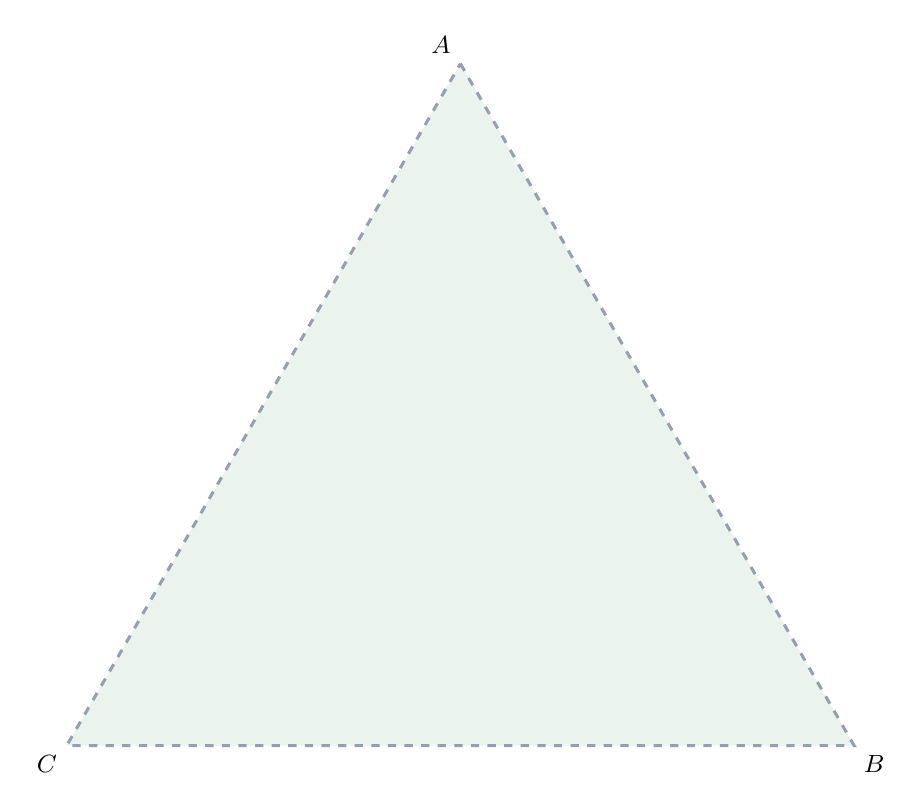
\begin{tikzpicture}
    \draw[dashed, xhline, line width=1.1pt, fill=xhgreen!10]
      (0,8.66) -- (5,0) -- (-5,0) -- cycle;
    \node[above left, font=\small] at (0,8.66) {\(A\)};
    \node[below right, font=\small] at (5,0) {\(B\)};
    \node[below left, font=\small] at (-5,0) {\(C\)};
  \end{tikzpicture}
  \end{center}
  \clearpage
  \thispagestyle{empty}%
  \begin{tikzpicture}[remember picture, overlay]
    \draw[dashed, xhline, line width=0.9pt]
      ([xshift=1.5cm]current page.north west) -- ([xshift=1.5cm]current page.south west);
    \node[rotate=90, font=\tiny, text=xhline]
      at ([xshift=1.5cm, yshift=-1.7cm]current page.north west) {裁切线};
  \end{tikzpicture}%
  \vspace*{15.0cm}
  \begin{center}
  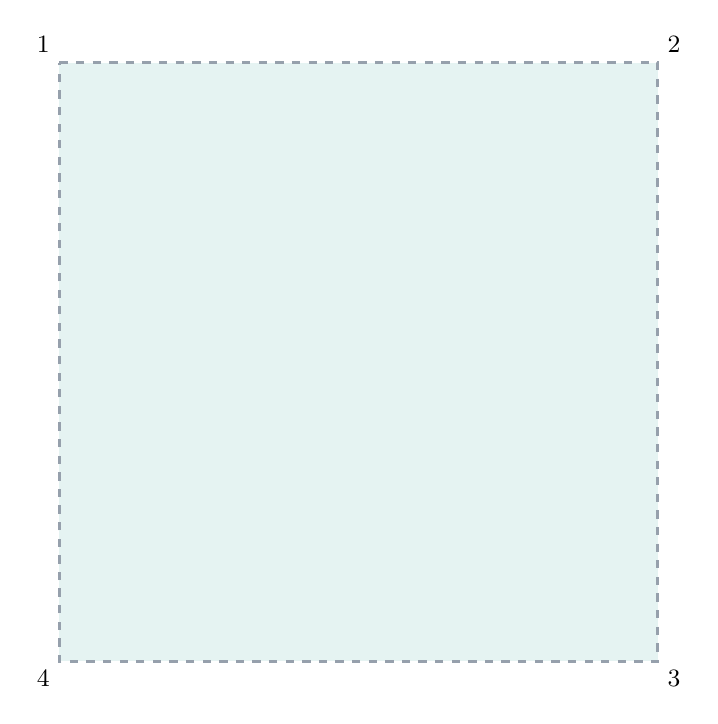
\begin{tikzpicture}
    \draw[dashed, xhline, line width=1.1pt, fill=xhteal!10]
      (-3.8,3.8) -- (3.8,3.8) -- (3.8,-3.8) -- (-3.8,-3.8) -- cycle;
    \node[above left, font=\small] at (-3.8,3.8) {\(1\)};
    \node[above right, font=\small] at (3.8,3.8) {\(2\)};
    \node[below right, font=\small] at (3.8,-3.8) {\(3\)};
    \node[below left, font=\small] at (-3.8,-3.8) {\(4\)};
  \end{tikzpicture}\\[5pt]
  {\songti\footnotesize
     （3）翻到这一面，沿正方形的轮廓，裁出一张正方形纸片。}
  \end{center}
  \clearpage
  \endgroup
}
% ---------------- 图片占位符 ----------------
\newcommand{\imgph}[2][4cm]{%
  \begin{center}%
  \begin{tikzpicture}%
    \node[draw=xhteal, densely dashed, line width=1pt, rounded corners=4pt,
          fill=xhteal!5!white, inner sep=8pt, align=center, text width=0.74\textwidth,
          minimum height=#1, font=\small]
      {\textcolor{xhteal}{\bfseries 【图片位置】}\\[4pt] #2};%
  \end{tikzpicture}%
  \end{center}%
}

% ---------------- 插图（与课件同名的命令，讲义里也能用）----------------
% 图放在 00-共享\图片\ 下，由上面的 \graphicspath 找到。
%      \imgfig{文件名}                  默认宽 0.72\textwidth
%      \imgfig[0.42\textwidth]{文件名}   指定宽度
\newcommand{\imgfig}[2][0.72\textwidth]{%
  \begin{center}%
    \includegraphics[width=#1]{#2}%
  \end{center}%
}

% ---------------- 表格行高（学生要往里写字，行抬高一些）----------------
\renewcommand{\arraystretch}{1.5}

% ---------------- 列表与行距 ----------------
\setlist[itemize]{itemsep=3pt,topsep=4pt,parsep=0pt,leftmargin=1.6em}
\setlist[enumerate]{itemsep=3pt,topsep=4pt,parsep=0pt,leftmargin=2.0em}
\linespread{1.28}